\documentclass{beamer}
\usetheme{Boadilla}
\usepackage{color}
\usepackage{multirow} 
\newcommand{\wf}{\color{white}}
\newcommand{\tf}{\color{black}}
\begin{document}
\title{Truth, Justice and Cake-Cutting}
\author{Alina Elterman}
\titlegraphic{
\includegraphics[scale=0.1]{bilder/HHU_Logo}}
%\institute{Institut f\"ur Informatik \\ $\:\:\:\:\:\:\:\:\:\:$Kryptologie und Komplexit\"atstheorie}
\date{\today}

\frame{\titlepage}

\frame{\frametitle{Inhaltsverzeichnis}\tableofcontents}


\section{Einleitung}
\frame{\frametitle{Cake-Cutting}
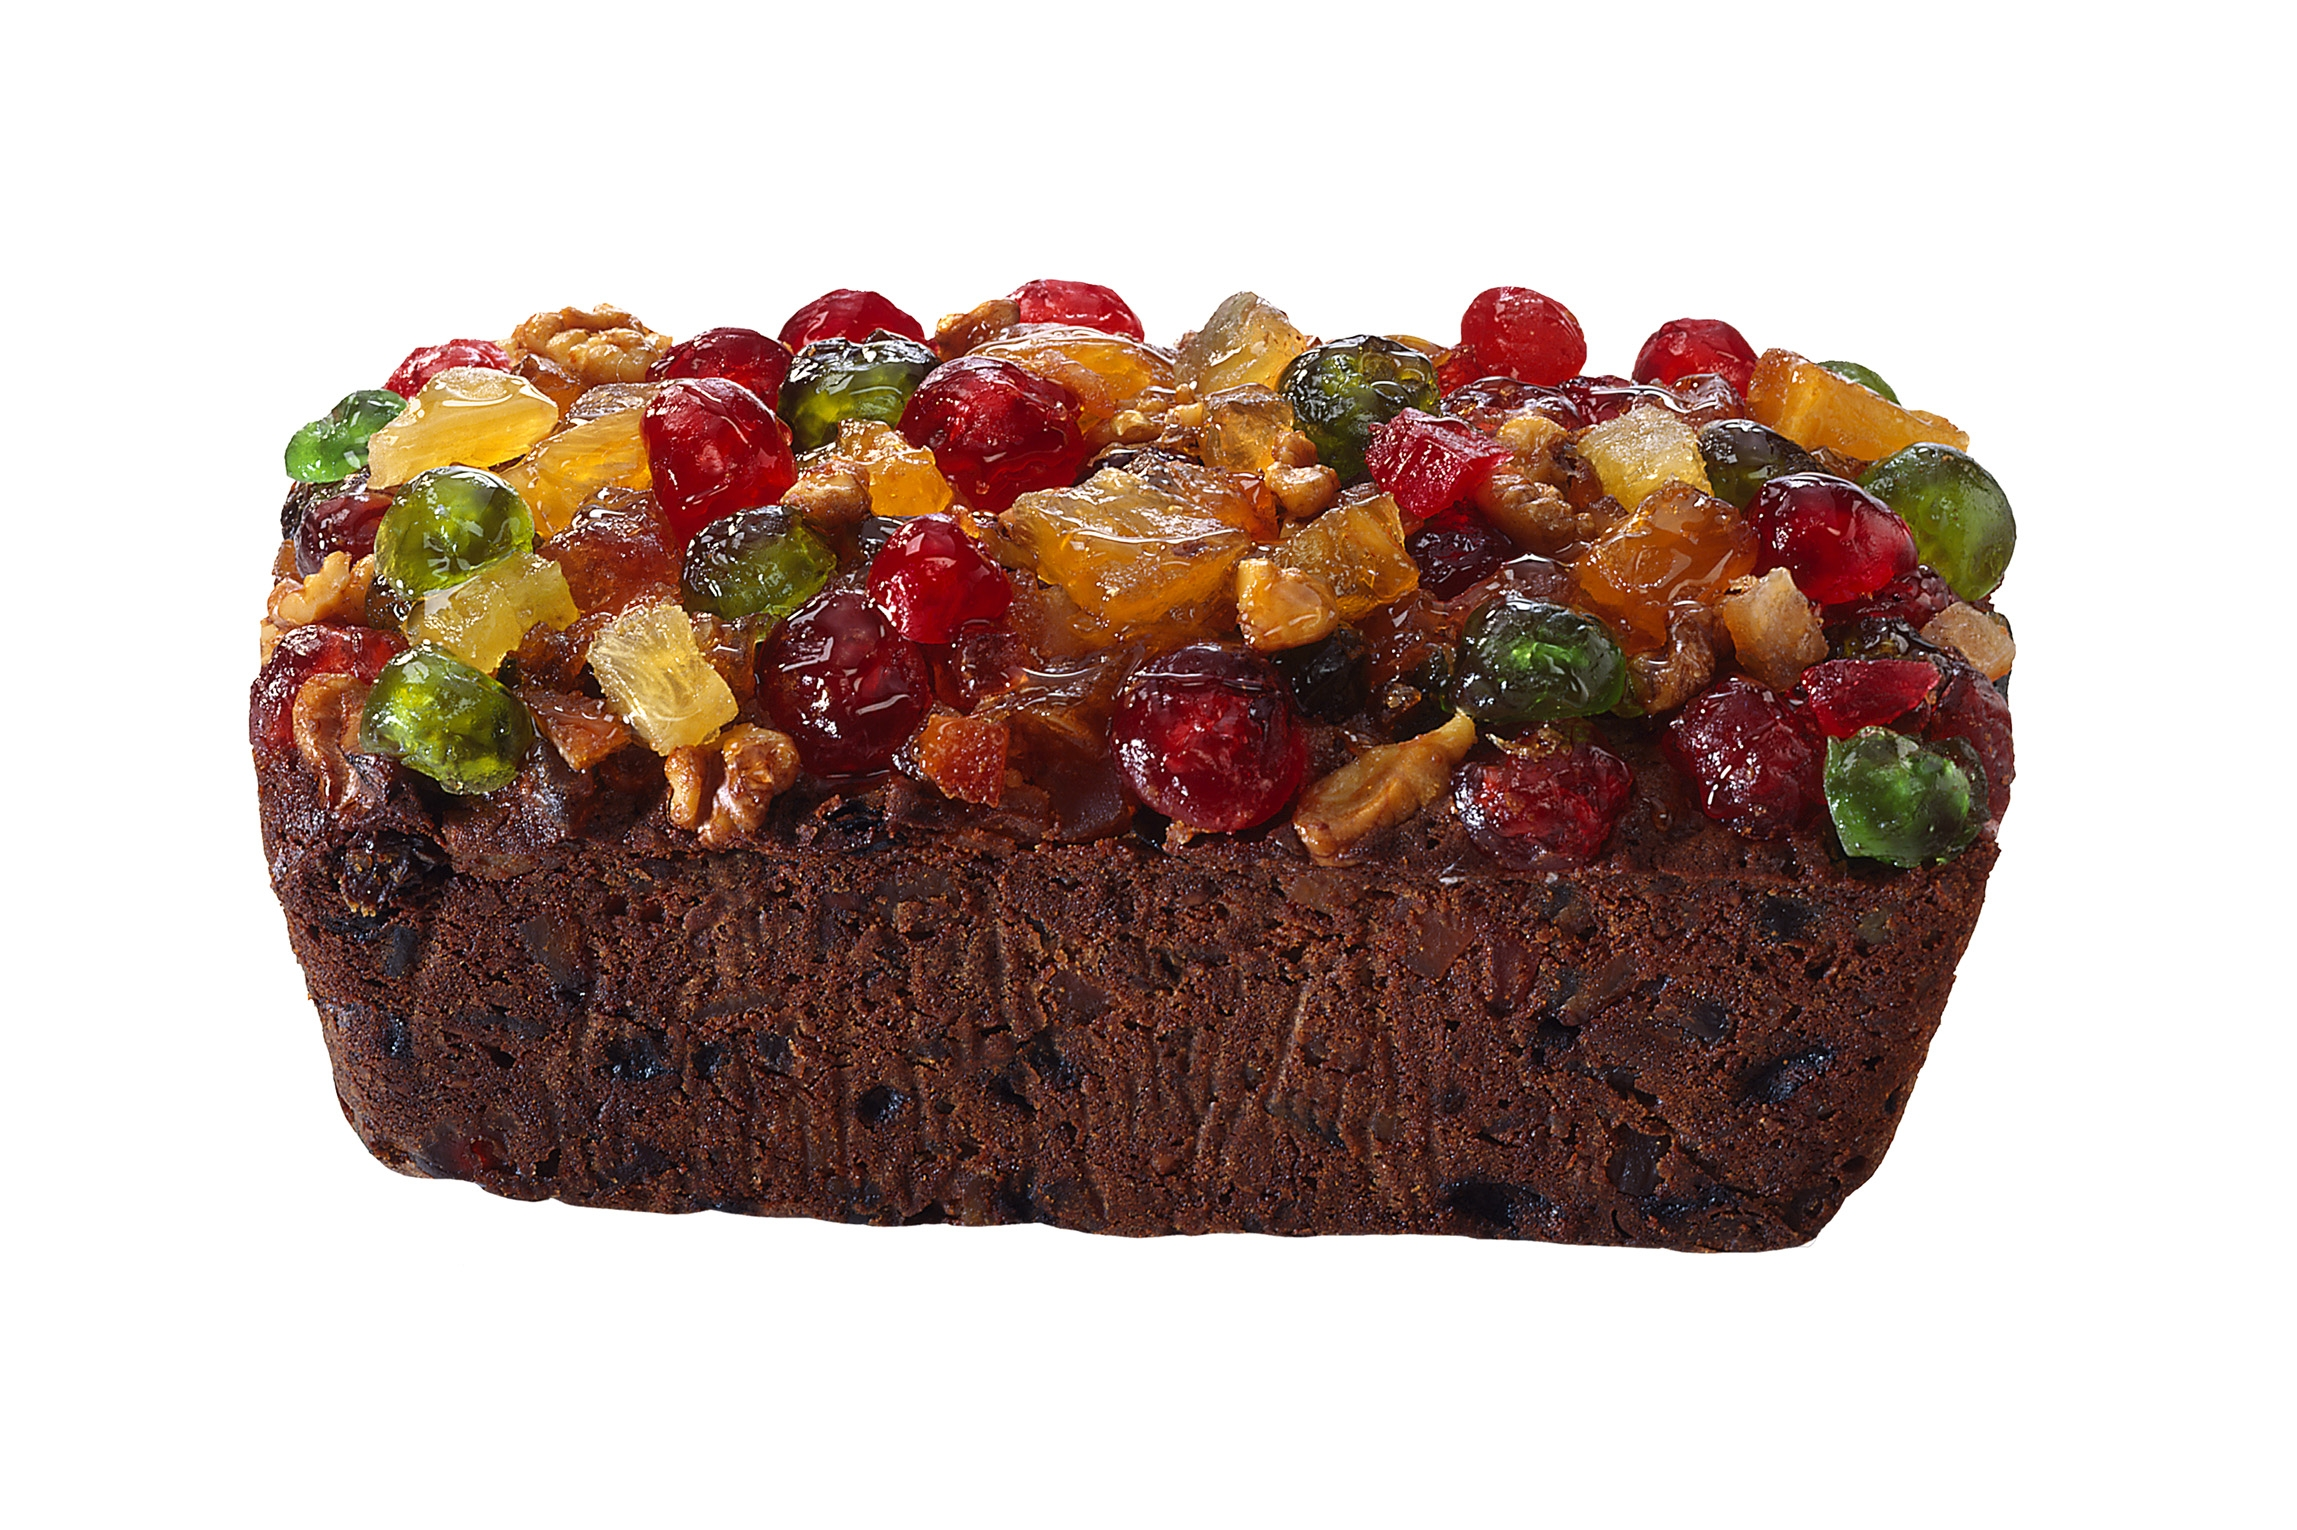
\includegraphics[scale=0.55]{fruitcake.jpg}\\
Kuchen - Metapher f\"ur ein beliebig oft teilbares Gut
}

\frame{\frametitle{Cake-Cutting}
\begin{itemize}
\item Aufteilung einer beliebig teilbaren Ressource zwischen $n$ Spielern
\item Schwerpunkt: Aufteilung erfolgt unter bestimmten Gerechtigkeitskriterien
\item Anwendungen: politische Konflikte, Scheidungen, Nachl\"asse, Aufteilung der Rechenzeit $\ldots$
\end{itemize}
}
\frame{\frametitle{Cake-Cutting}
\begin{tabular}{cc} 
  \multirow{3}{*}{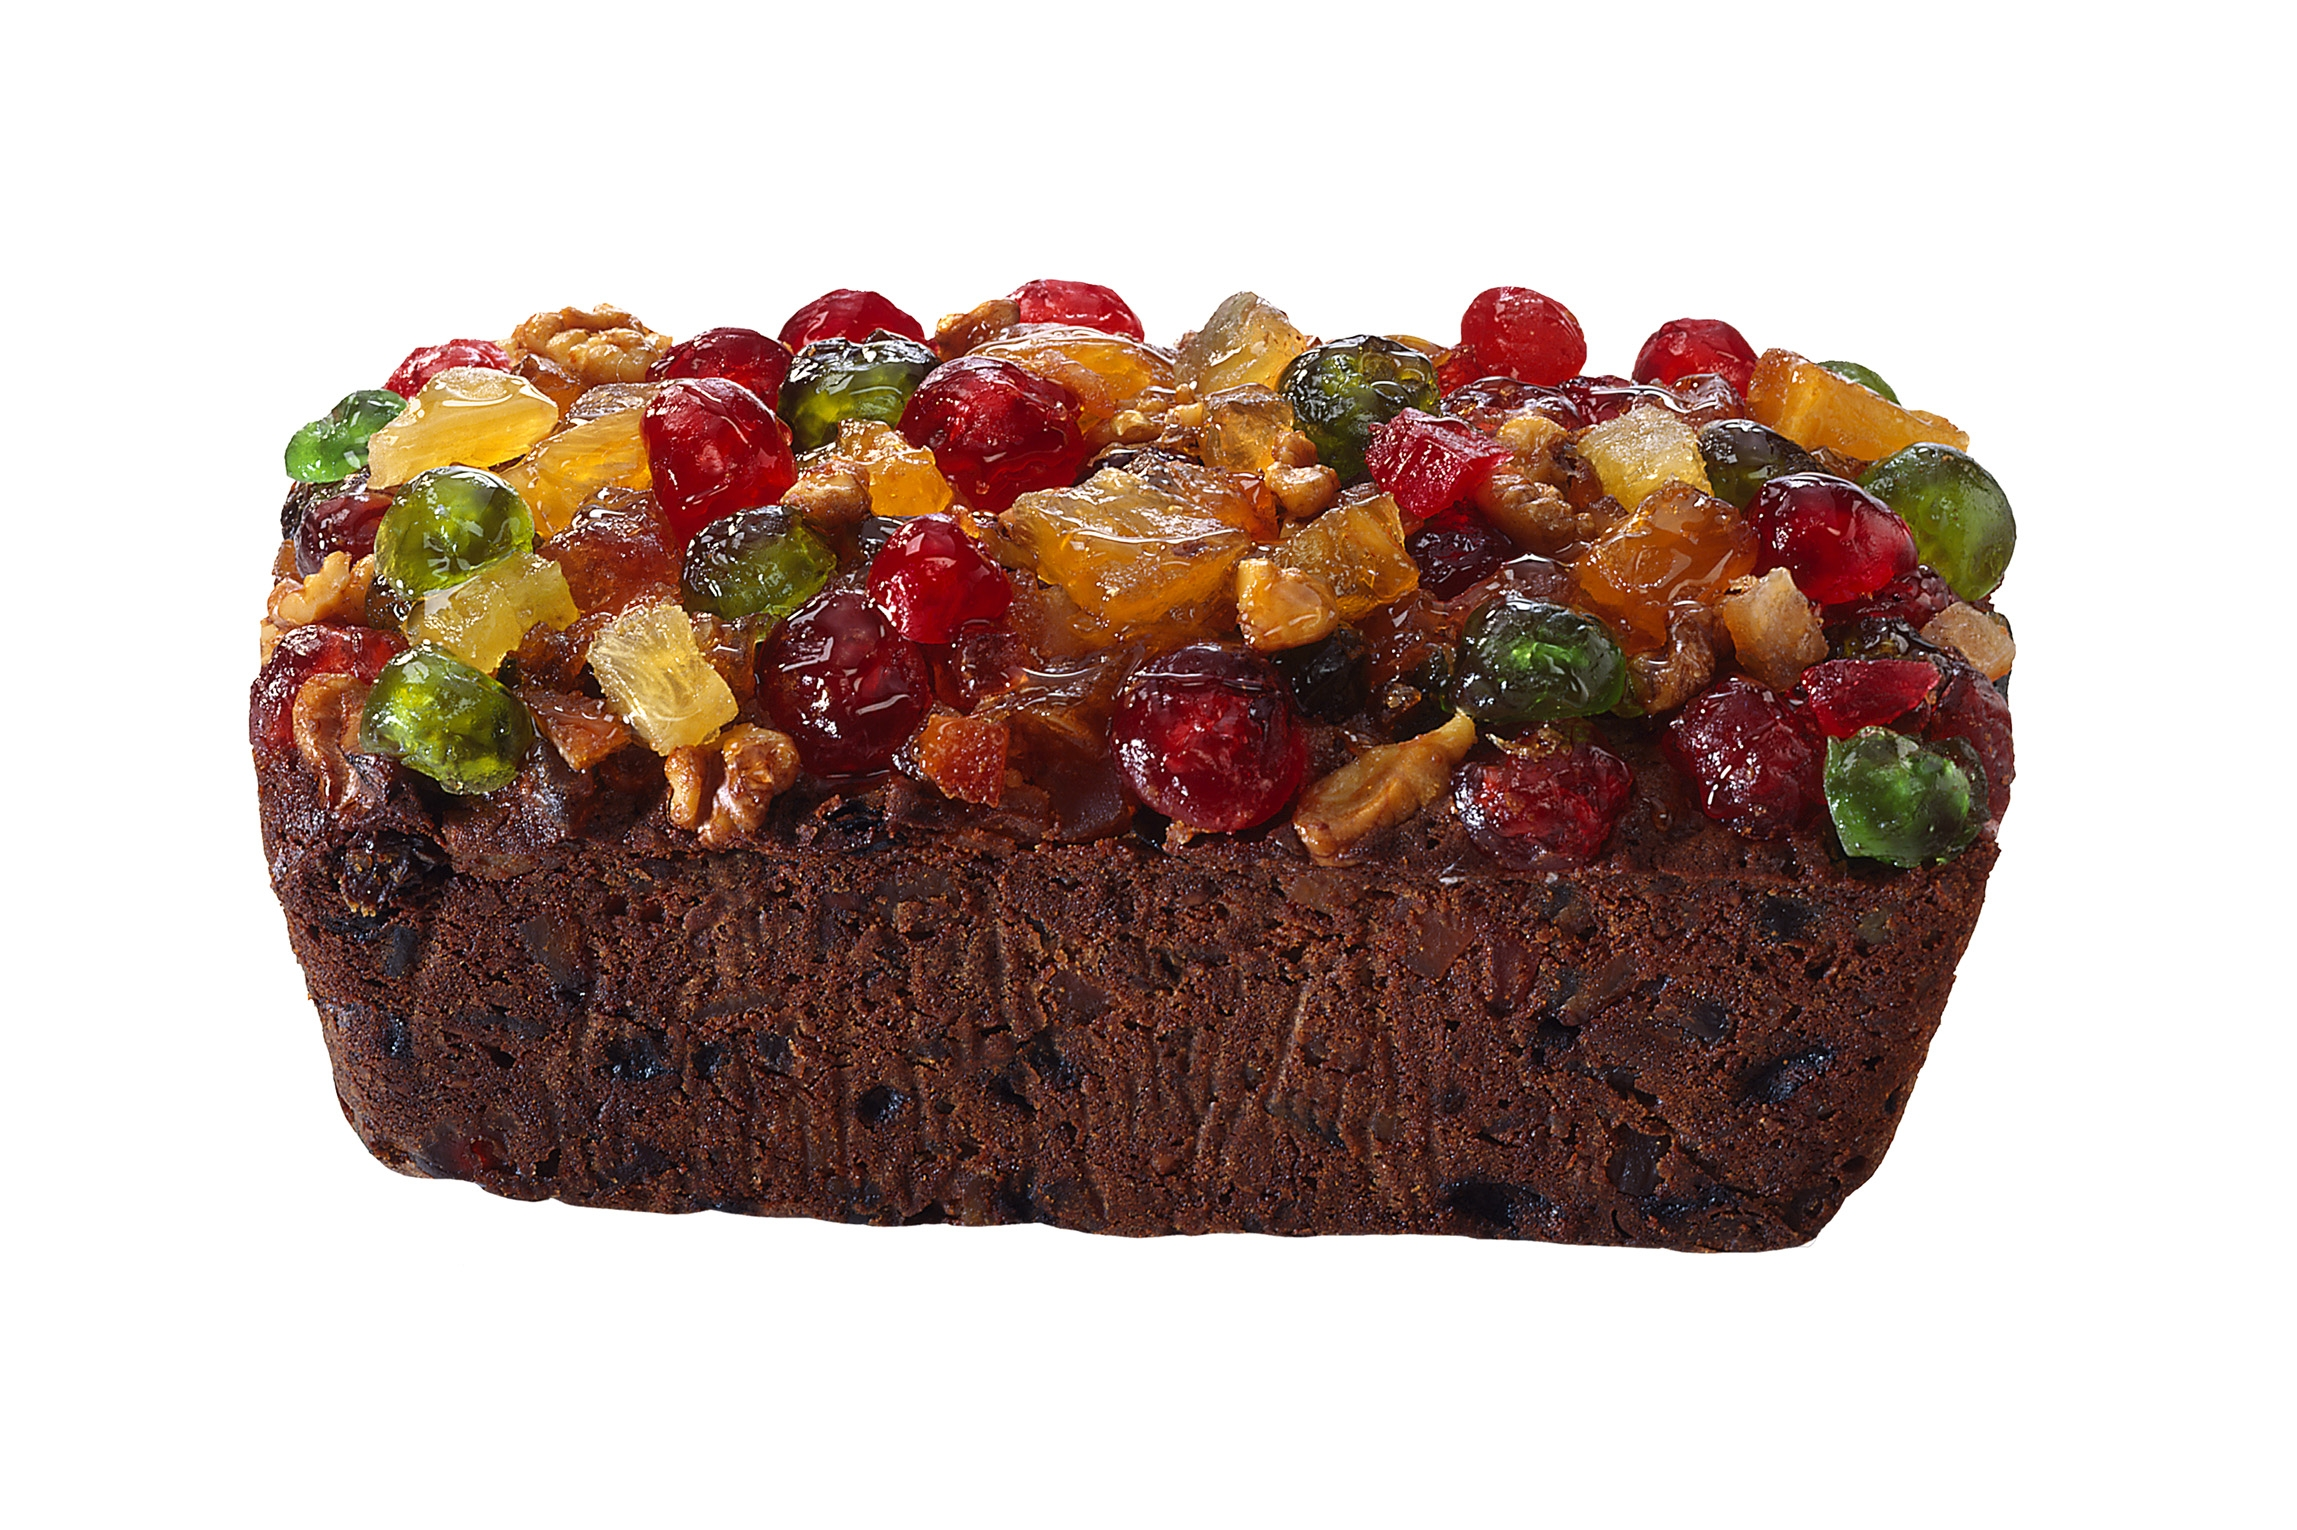
\includegraphics[scale=0.35]{fruitcake.jpg}} & 
\includegraphics[scale=0.30]{rei.jpg}\\& \textcolor{white}{Ich mag Kirschen!}\\ &
\includegraphics[scale=0.25]{ami.jpg}\\& \textcolor{white}{Ich mag Ananas!}\\
  &
\includegraphics[scale=0.25]{bunny.jpg} \\& \textcolor{white}{Ich habe Hunger!} \\
\end{tabular} 
\newline
\textcolor{white}{\textbf{Die Pr\"aferenzen auf bestimmte St\"ucke k\"onnen sich unterscheiden!}
}}
\frame{\frametitle{Cake-Cutting}
\begin{tabular}{cc} 
  \multirow{3}{*}{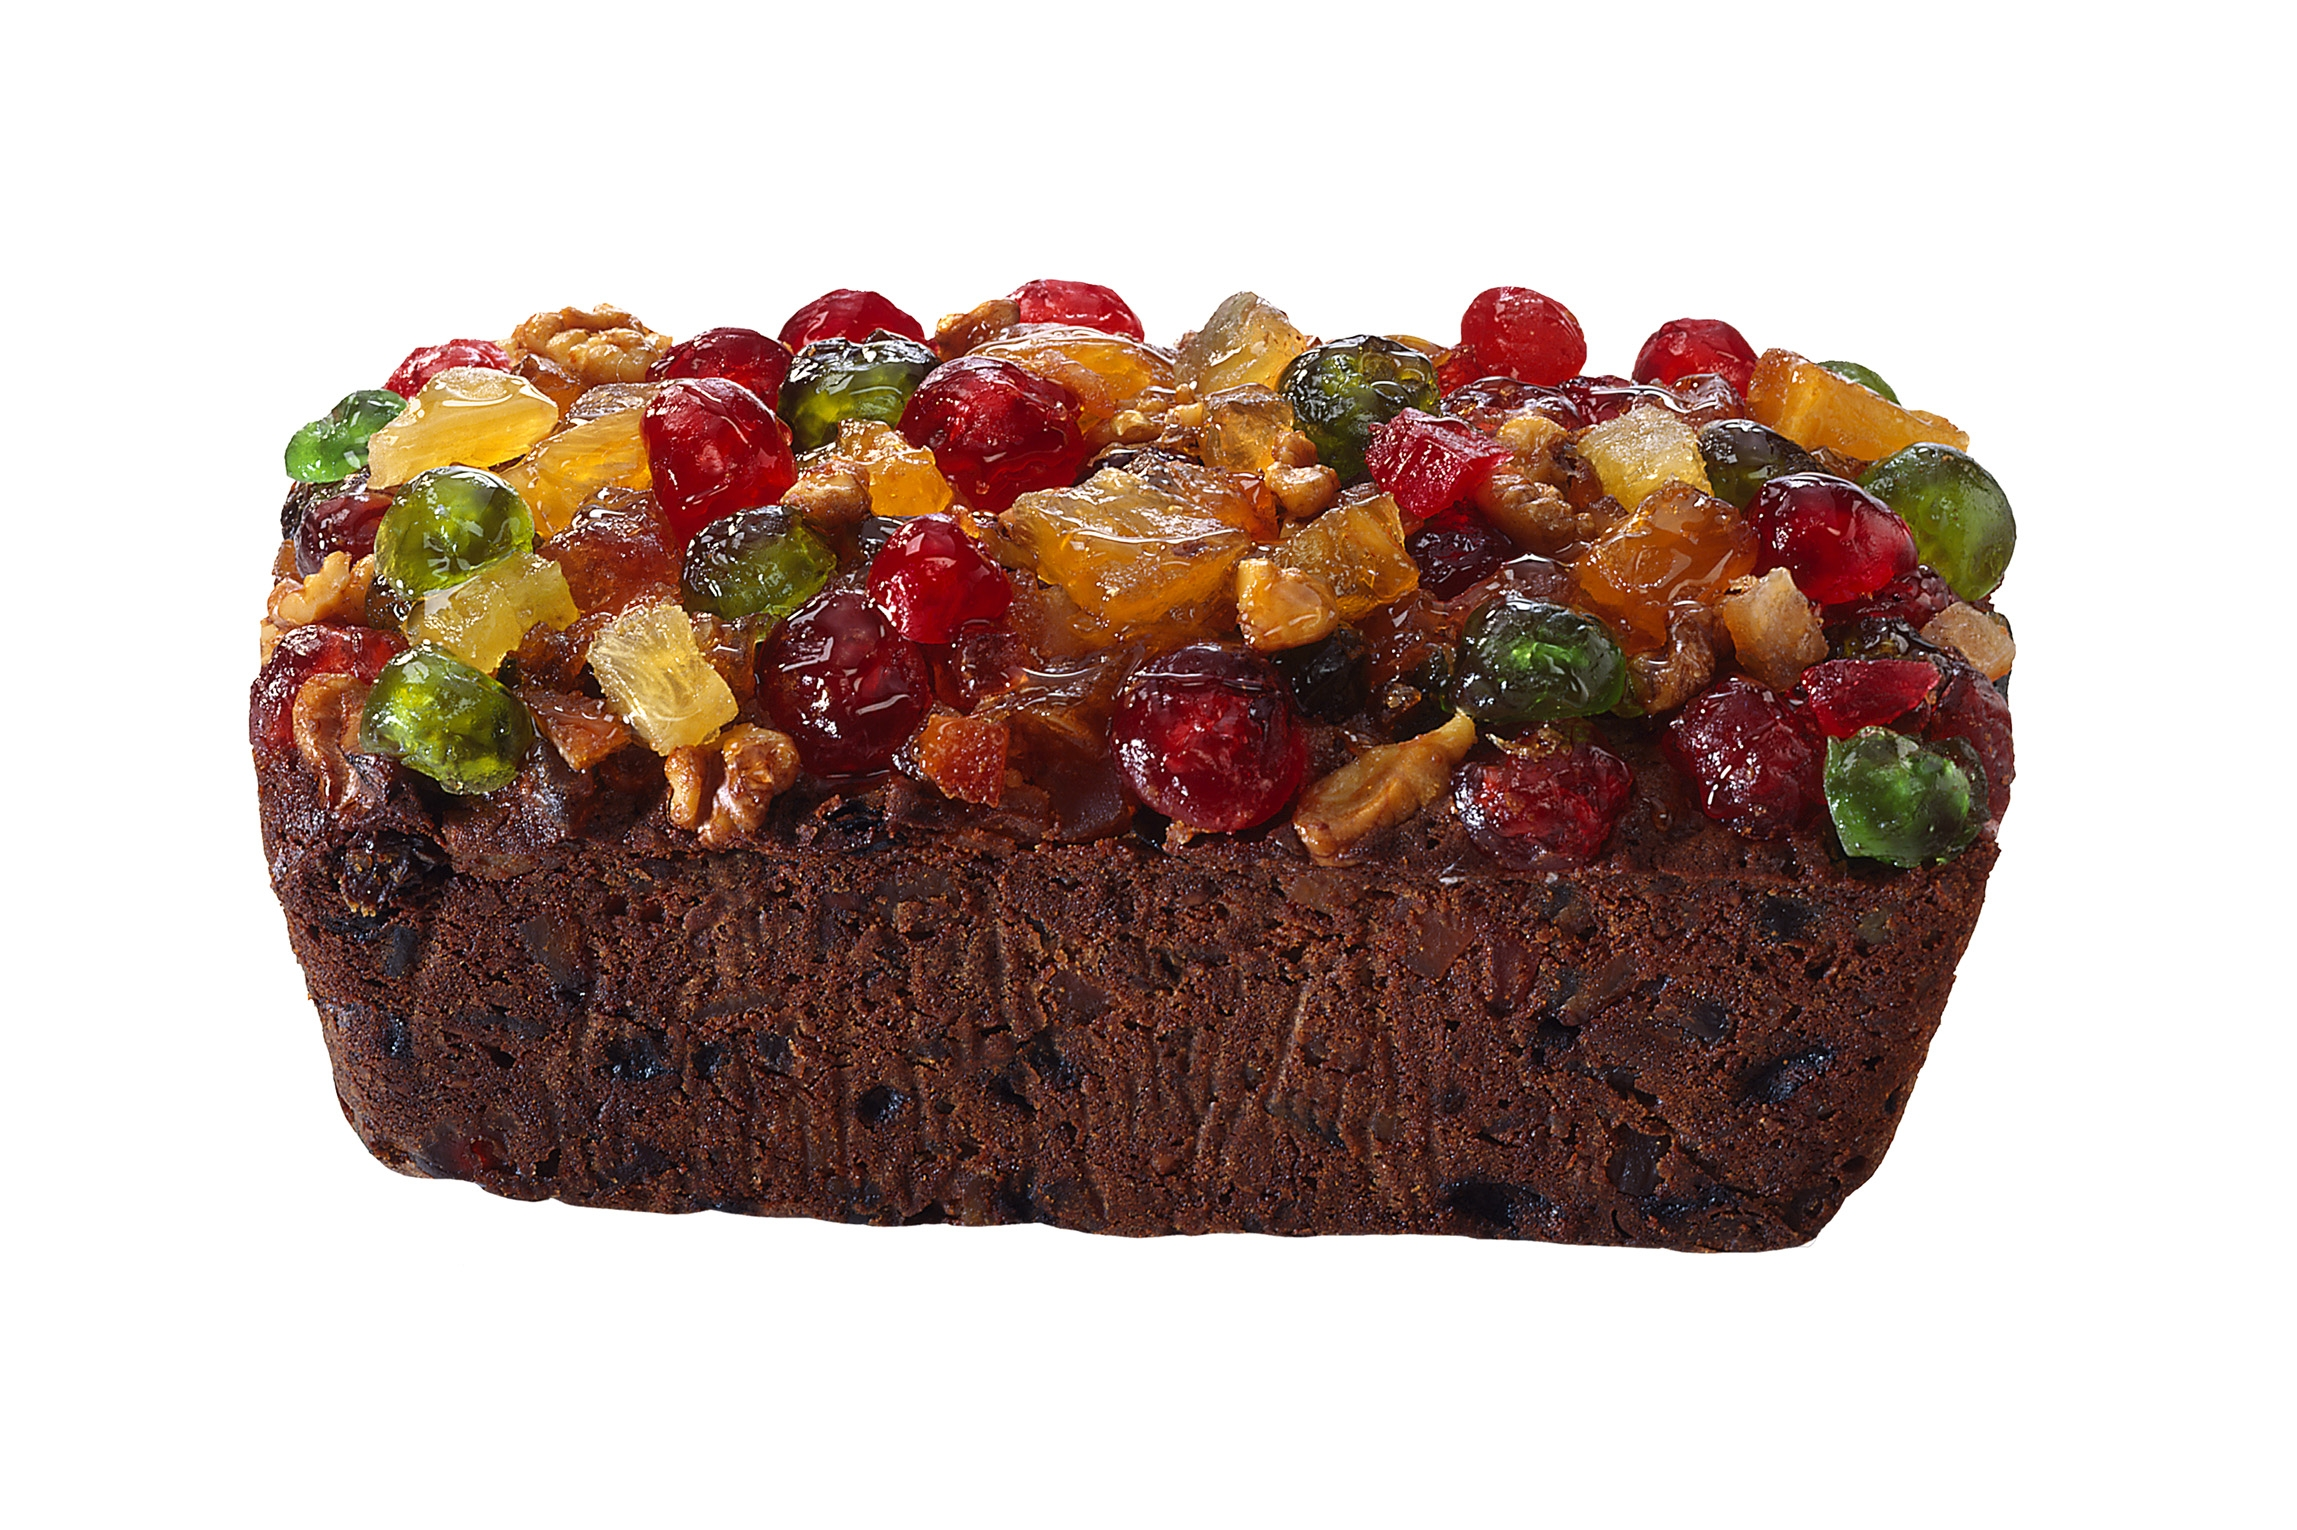
\includegraphics[scale=0.35]{fruitcake.jpg}} & 
\includegraphics[scale=0.30]{rei.jpg}\\& Ich mag Kirschen!\\ &
\includegraphics[scale=0.25]{ami.jpg}\\& Ich mag Ananas!\\
  &
\includegraphics[scale=0.25]{bunny.jpg} \\& Ich habe Hunger! \\

\end{tabular} \pause
\newline
\textbf{Die Pr\"aferenzen auf bestimmte St\"ucke k\"onnen sich unterscheiden!}
}

\section{Grundbegriffe}
\subsection{Der Kuchen und die Bewertung}
\frame{\frametitle{Grundbegriffe}
\begin{itemize}
\item $P_n$=$\{p_1,...,p_n\}$ - Menge von $n$ Spieler
\item Intervall $X=[0,1]$ - einziges, heterogenes, beliebig teilbares Gut
(Kuchen)\pause
\item Bewertungsfunktion - subjektive und geheime Funktion, die jedem Spieler f\"ur jedes St\"uck einen Nutzwert zuordnet\pause
\item Gesucht: Aufteilung $X_1, \ldots , X_n$ mit $X_i$ St\"uck von $p_i$ und $\sideset{}{ }\bigcup\limits_{i=1}^{n}X_i=X$
\end{itemize}\pause
\textcolor{red}{Es werden komplette Aufteilungen mit beliebigen Bewertungsfunktionen betrachtet!}
}

\frame{\frametitle{Gerechtigkeitskriterien}
\begin{itemize}
\item{\textbf{Proportionalit\"at}
\newline Jeder Spieler bekommt (nach seiner Bewertung)
    mind. $\frac{1}{n}$ des Kuchens.}
\item{\textbf{Neidfreiheit}
\newline Kein Spieler bewertet ein fremdes St\"uck besser als sein Eigenes.}
%\item{\textbf{Exaktheit}
%\newline Jeder Spieler bekommt (nach seiner Bewertung)
 %   ein identisches St\"uck bzgl. der Gr\"o\'se.}
\end{itemize}
}
\frame{\frametitle{Protokoll}
\begin{itemize}
\item Bestimmt wie die Aufteilung zur Stande kommt
\item Besteht aus Regeln und Strategien
\item Die Prozedur kennt die Bewertungsfunktionen der Spieler nicht, erfragt diese aber durch die Regeln.
\end{itemize}

}

\frame{\frametitle{Strategiesicherheit}
\"Ublicherweise f\"ur Cake-Cutting:
\newline Protokoll ist \emph{strategiesicher}:\\
 Es gibt mind. \textbf{einen} Fall, wo der Spieler durch Unehrlichkeit kein wervolleres St\"uck bekommt.\pause
\newline
\newline
Genannt: \emph{schwache Strategiesicherheit}
}

\frame{\frametitle{Strategiesicherheit}
In der Social Choice Theorie:
\newline Protokoll ist \emph{strategiesicher}: \\
In \textbf{keinem} Fall, bekommt ein Spieler durch Unehrlichkeit ein wertvolleres St\"uck.\\\pause
\textbf{L\"ugen bringt NIEMALS einen Vorteil!}
}


\frame{\frametitle{Cut $\&$ Choose}
\begin{tabular*}{\textwidth}{|@{\extracolsep{\fill}}l|c|r|}
\hline
\textbf{Regeln}& \textbf{Strategie von $p_1$}& \textbf{Strategie von $p_2$}\\
\hline
1. Spieler $p_1$ teilt &Teile den Kuchen in zwei&\\
den Kuchen in zwei&gleich wertvolle St\"ucke&\\
St\"ucke&&\\
\hline
2. Spieler $p_2$ w\"ahlt&&W\"ahle das \\
Eines aus&&wertvollere St\"uck\\
\hline
3. Spieler $p_1$ bekommt &&\\das \"Ubrige&&\\
\hline
\end{tabular*}\\}
\frame{\frametitle{Strategiesicherheit gilt nicht bei Cut $\&$ Choose}
\begin{figure}[!h]
\centering
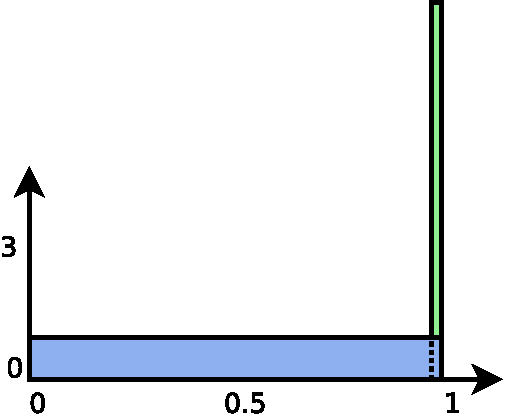
\includegraphics[width=5cm]{cc.pdf}
\end{figure}
}

\section{Paper}
\frame{\frametitle{Resultat von Y. Chen, J. Lai, D. Parkes
und A. Procaccia}
Entwurf von einem polynomialzeit Algorithmus der proportional, neidfrei und stark strategiesicher ist.
}

\subsection{Vorraussetzungen f\"ur den Algorithmus}
\frame{\frametitle{Einschr\"ankungen von Cake-Cutting}
Das Entsorgungsargument:\\
Teile vom Kuchen d\"urfen entfernt werden.\\
\pause
\textbf{NEU:} Aus Neidfreiheit folgt nicht mehr die Proportionalit\"at. (zuvor ja! ) 
}
\frame{\frametitle{St\"uckweise gleiche Bewertung}
\begin{figure}[!h]
\centering
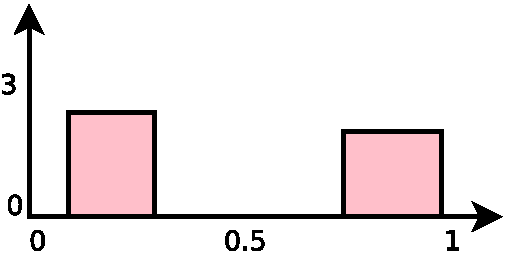
\includegraphics[width=5cm]{keinuniform.pdf}\pause
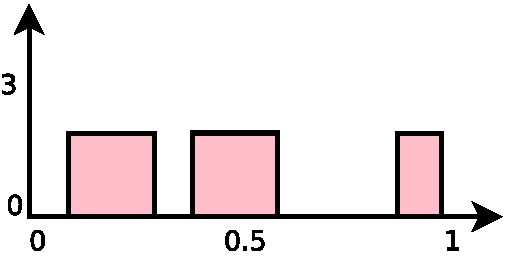
\includegraphics[width=5cm]{uniform.pdf}
\end{figure}\pause
KEINE St\"uckweise gleiche Bewertung!

}

\subsection{Beispiel}

\frame{\frametitle{Algorithmusidee}
\begin{itemize}
\item Finde eine Menge von Spielern mit der am dichtesten bewerteten Fl\"ache
\item Teile diese auf
\item Wiederhole bis jeder Spieler ein St\"uck hat und entsorge den Rest des Kuchens
\end{itemize}
}

\frame{\frametitle{Alle unterschiedlich}
\begin{figure}[!h]
\centering
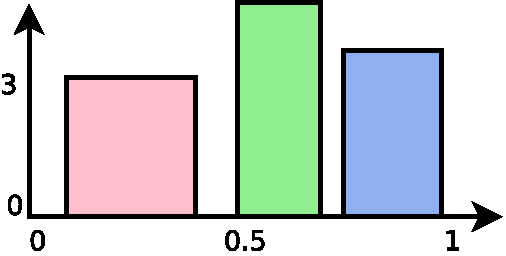
\includegraphics[width=5cm]{bsp1.pdf}
\end{figure}
}
\frame{\frametitle{Zwei gleich}
\begin{figure}[!h]
\centering
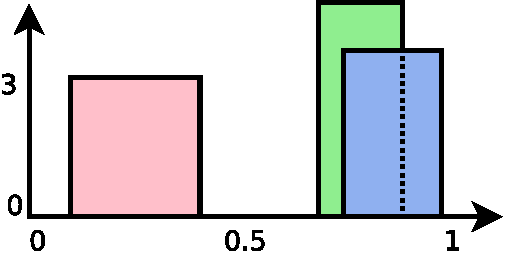
\includegraphics[width=5cm]{bsp2.pdf}
\end{figure}\pause
L\"ange $X_2=0.2$ und L\"ange $X_3=0.25$. 
}
\frame{\frametitle{Drei gleich Fall.1}
\begin{figure}[!h]
\centering
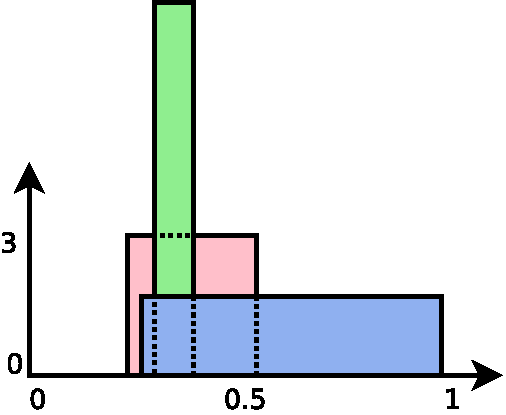
\includegraphics[width=5cm]{bsp4.pdf}
\end{figure}\pause
L\"ange $X_2=0.1$,L\"ange $X_2=0.3$ und L\"ange $X_3=0.25$. 
}
\frame{\frametitle{Drei gleich Fall.2}
\begin{figure}[!h]
\centering
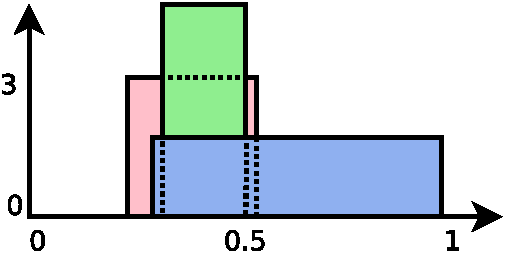
\includegraphics[width=5cm]{bsp3.pdf}
\end{figure}\pause
L\"ange $X_3=0.25$, L\"ange $X_2 \& X_3=0.22$ und L\"ange $X_2 \& X_3 \& X_1=0.2$,
}



\frame{\frametitle{Fragen:}
\begin{itemize}
\item Kann man Cake-Cutting weniger einschr\"anken um das selbe Resultat zu erreichen?\pause \newline Y. Chen, J. Lai, D. Parkes und A. Procaccia wollen zun\"achst das Entsorgungsargument beseitigen.\pause
\item Unter welchen Einschr\"ankungen gibt es neidfreie Algorithmen? 
\end{itemize}
}

\frame{\frametitle{}
Vielen Dank f\"ur die Aufmerksamkeit!
}


\section{Quellenverzeichnis}
\frame{\frametitle{Quelle:}[CLPP10] Y. Chen, J. Lai, D. Parkes
und A. Procaccia: Truth, Justice and Cake Cutting. \emph{AAAI-10: Proc. 24th AAAI Conference on Artificial Intelligence}, pp. 756-761, Jul 2010.
}

%\section{Proof}
%\frame{\frametitle{Every envy-free allocation is proportional}
%\begin{itemize}
%\item[Proof] by contradiction:\\ Assume $A$ is an envy-free allocation, but not proportional. From envy-freeness follows $v_i(X_i) \geq v_i(X_j)$ for each pair of players $p_i, p_j \in P_n$ and so each player has at least an as much valuable piece of cake as each other player. Hereby each player owns in his own valuation at least as much as $(n-1)$ other players and so at least $1/n$. WS!! The allocation $A$ is proportional. %$\lightning$ 
%\\Therefore, all envy-free allocations are proportional.
%\end{itemize}
%}


\end{document}